\section{Introduction}
\label{sec:introduction}

Example of a citation~\cite{latexcompanion}.

\lipsum[1]

\begin{figure}
    \centering
    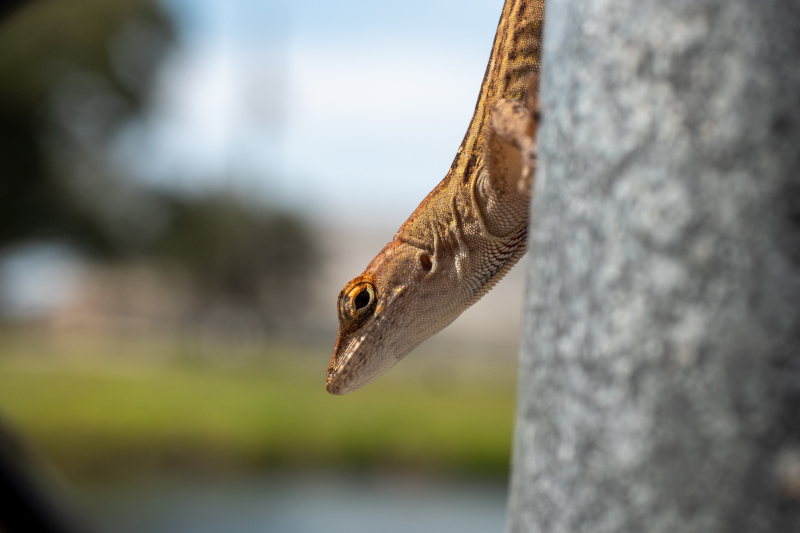
\includegraphics[width=0.8\textwidth]{assets/graphics/example.jpg}
    \caption{A picture I took a while ago!}
    \label{fig:test-figure}
\end{figure}


\section{Methods and tools}
\label{sec:methods-and-tools}

\subsection{Subsection 1}
\label{subsec:subsec1}

\lipsum[1]

\subsection{Subsection 2}
\label{subsec:subsec2}

\lipsum[2]

\subsubsection{Subsubsection 1}
\label{subsubsec:subsubsec-1}

Hello World!
Some math? \(\begin{bmatrix}
                 1 & 2 \\
                 3 & 4
\end{bmatrix}\)

\subsubsection{Subsubsection 2}
\label{subsubsec:subsubsec-2}

\lipsum[6]

\subsection{Subsection 3}
\label{subsec:subsec3}

\lipsum[3]


\section{Results}
\label{sec:results}

\lipsum[2]

\subsection{Subsection 1}
\label{subsec:subsec12}

\lipsum[3-6]

\subsection{Subsection 2}
\label{subsec:subsec13}

\lipsum[7-10]


\section{Discussion}
\label{sec:discussion}

\lipsum[1-2]

\subsection{Subsection 1}
\label{subsec:subsec123}

\lipsum[2-3]

\subsection{Subsection 2}
\label{subsec:subsec134}

\lipsum[11-12]


\section{Summary}
\label{sec:summary}

\lipsum[1-3]
